\documentclass[11pt]{article}

\usepackage[margin=2cm,a4paper]{geometry}
\usepackage{amsmath}
\usepackage{amssymb}
\usepackage{booktabs}
\usepackage{graphicx}
\usepackage{array}
\usepackage[hidelinks]{hyperref}

% ... complementarity symbol
\newcommand{\comp}{\perp}
% ... AMPL name typeset in a monospaced font
\newcommand{\ampl}[1]{\texttt{#1}}
% ... positive and negative parts of the flow
\newcommand{\qp}{q^{+}}
\newcommand{\qn}{q^{-}}

\title{Water Distribution Network Design Tutorial: Background\\NOMICC School 2026}
\author{Sven Leyffer, assisted by {\tt claude}}
\date{\today}

\begin{document}
\maketitle

\section{Overview}

We consider two mathematically equivalent formulations of a water
distribution network design problem (one with binary variables and one
with complementarity constraints). The problem is to
choose the diameter of each pipe and the flow through it so as to meet the
consumer demand at minimum cost, where the cost combines the pumping/water cost
at the reservoirs, the investment cost of the pipes, and a small penalty on the
total flow.

The physical constraints include flow-conservation constraints, and pressure-loss
constraints. Initially, we will treat the pipe diameter as continuous, and then
develop an integer model (using SOS-1 constraints). We will consider two networks,
a small $8$-node network and a larger $28$-node network. The networks are shown in
Figure~\ref{fig:water}.

\begin{figure}[htbp]
  \centering
  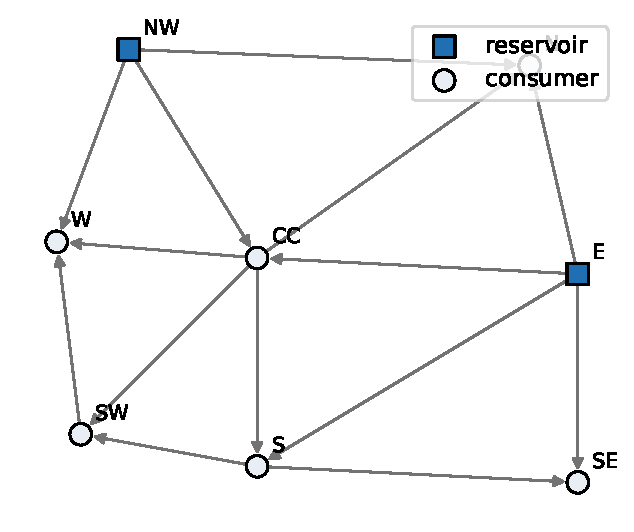
\includegraphics[width=0.48\textwidth]{figures/water01.pdf}\hfill
  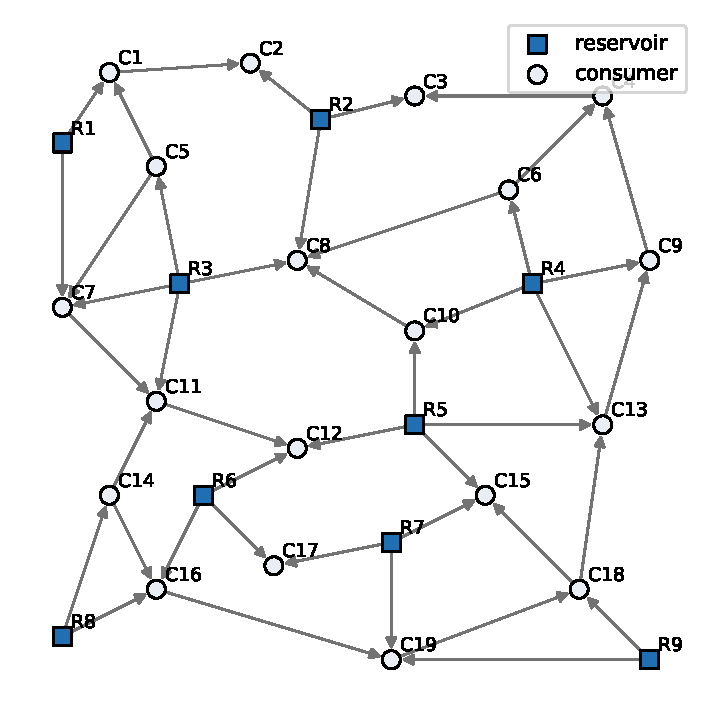
\includegraphics[width=0.48\textwidth]{figures/water02.pdf}
  \caption{Small network (left) with $8$ nodes ($2$ reservoirs \ampl{NW},
    \ampl{E}; $6$ consumers) and $14$ arcs, and larger network (right) $28$ nodes ($9$ reservoirs
    \ampl{R1}--\ampl{R9}; $19$ consumers \ampl{C1}--\ampl{C19}) and $44$ arcs.
    Squares are reservoirs, circles are consumers; each arrow shows the reference
    orientation $i\to j$ of an arc. Coordinates are in meters (small) and km (large).}
  \label{fig:water}
\end{figure}

We will work from {\tt AMPL} models that are also provided as reference (but never used), see Table~\ref{tab:ref-ampl}. You can run these models on the NEOS server, \url{https://neos-server.org/neos/}

\section{Sets, parameters, and constants}

The model is defined over the following sets (with {\tt AMPL} for reference purposes only)
\begin{center}
\begin{tabular}{ll@{\qquad}l}
  \toprule
  Symbol & AMPL name & Description \\
  \midrule
  $\mathcal{N}$ & \ampl{nodes}      & set of nodes \\
  $\mathcal{R}$ & \ampl{reservoirs} & reservoir nodes, $\mathcal{R}\subseteq\mathcal{N}$ \\
  $\mathcal{C}$ & \ampl{consumers}  & consumer nodes, $\mathcal{C}\subseteq\mathcal{N}$ \\
  $\mathcal{A}$ & \ampl{arcs}       & arcs (pipes), $\mathcal{A}\subseteq\mathcal{N}\times\mathcal{N}$ \\
  $\mathcal{D}$ & -- & pipe diameters, see Table~\ref{tab:diameters} \\
  \bottomrule
\end{tabular}
\end{center}

\newcommand{\Qpow}{Q_{\text pow}}
The data associated with each node $i\in\mathcal{N}$ are:
$D_i$ (\ampl{demand}), $H_i$ (\ampl{height}), $(x_i,y_i)$, $S_i$ (\ampl{supply}),
$C^{w}_i$ (\ampl{wcost}), and $C^{p}_i$ (\ampl{pcost}) (the concrete values are listed in the
data files and the networks are illustrated in Figure~\ref{fig:water}).
The remaining constants are scalar or derived quantities, summarized in
Table~\ref{tab:constants}. We assume that {\tt qpow = 2} (denoted by $\Qpow$) in the pressure-loss equation, so that we can write
\begin{equation}\label{eq:PL}
  q_{ij}^{\Qpow} = q_{ij} | q_{ij}|,
\end{equation}
see {\tt waterNLP.mod}. A similar equation can be constructed for any power $\Qpow\geq 2$. What can you say about the smoothness of this term?

\begin{table}[htbp]
  \centering
  \caption{Scalar and derived constants (identical in both models).}
  \label{tab:constants}
  \begin{tabular}{l l l >{\raggedright\arraybackslash}p{3.6cm} l}
    \toprule
    Symbol & AMPL name & Value / definition & Description & Units \\
    \midrule
    $P_{\text{loss}}$ & \ampl{dpow}  & $5.33$                  & power on diameter in pressure loss & --- \\
    $d_{\min}$ & \ampl{dmin}  & $0.15$                       & minimum pipe diameter              & m \\
    $d_{\max}$ & \ampl{dmax}  & $2.00$                       & maximum pipe diameter              & m \\
    $H_{\text{loss}}$ & \ampl{hloss} & $1.03\times10^{-3}$   & constant in pressure-loss equation & --- \\
    $C_d$      & \ampl{dprc}  & $6.90\times10^{-2}$          & scale factor in investment cost    & --- \\
    $P_{\text{cost}}$ & \ampl{cpow}  & $1.29$                & power on diameter in cost          & --- \\
    $\Qpow$ & \ampl{Qpow}  & $2.0$                & power constant in pressure-loss          & --- \\
    $R$        & \ampl{r}     & $0.10$                       & annual interest rate                      & --- \\
    $Q$        & \ampl{maxq}  & $2.00$                       & bound on $\qp$ and $\qn$           & m$^3$/s \\
    \addlinespace
    $d_{\text{avg}}$ & \ampl{davg} & $\sqrt{d_{\min}\,d_{\max}}$ & average (geometric mean) diameter & m \\
    $\rho$ & \ampl{rr} & $\dfrac{\sum_{i\in\mathcal{C}} D_i}{\sum_{i\in\mathcal{R}} S_i}$ & demand-to-supply ratio & --- \\
    $L_{ij}$ & \ampl{dist} & $\sqrt{(x_i-x_j)^2+(y_i-y_j)^2}$ & arc length, $(i,j)\in\mathcal{A}$ & m \\
    $\underline{h}_i$ & \ampl{hl} & $H_i+\!\begin{cases}7.5+5\,D_i & i\in\mathcal{C}\\ 0 & \text{otherwise}\end{cases}$ & minimum pressure head at node $i$ & m \\
    \bottomrule
  \end{tabular}
\end{table}

\paragraph{Notation convention.}
In the AMPL models, we use the construct \ampl{if i in reservoirs then s[i]},
which appears in the flow balance.  In the mathematical formulation we write the term
$\mathbf{1}[i\in\mathcal{R}]\,s_i$, i.e.\ the supply $s_i$ is added only at
reservoir nodes.

\clearpage
\section{Problem formulation}
\label{sec:minlp}

The MINLP uses a binary variable $z_{ij}$ per arc to indicate the flow direction:
positive flow $\qp_{ij}$ is allowed when $z_{ij}=1$ and negative flow $\qn_{ij}$
when $z_{ij}=0$.  The decision variables are listed in Table~\ref{tab:vars-minlp}. The pipe diameters are listed in Table~\ref{tab:diameters} (we will treat $d_{ij}$ as continuous initially), and the correspondence between {\tt AMPL} and math equations is in Table~\ref{tab:ref-minlp}.

\begin{table}[htbp]
  \centering
  \caption{Decision variables of the MINLP.}
  \label{tab:vars-minlp}
  \begin{tabular}{l l l l l}
    \toprule
    Symbol & AMPL name & Index & Bounds & Description \\
    \midrule
    $\qp_{ij}$ & \ampl{qp} & $(i,j)\in\mathcal{A}$ & $[0,\,Q]$ & positive flow on arc (m$^3$/s) \\
    $\qn_{ij}$ & \ampl{qn} & $(i,j)\in\mathcal{A}$ & $[0,\,Q]$ & negative flow on arc (m$^3$/s) \\
    $d_{ij}$  & \ampl{d}  & $(i,j)\in\mathcal{A}$ & $[d_{\min},\,d_{\max}]$ & pipe diameter (m) \\
    $h_i$     & \ampl{h}  & $i\in\mathcal{N}$     & $\ge \underline{h}_i$ & pressure head at node (m) \\
    $s_i$     & \ampl{s}  & $i\in\mathcal{R}$     & $[0,\,S_i]$ & supply at reservoir (m$^3$/s) \\
    $z_{ij}$  & \ampl{z}  & $(i,j)\in\mathcal{A}$ & $\{0,1\}$ & flow-direction selector \\
    \bottomrule
  \end{tabular}
\end{table}

\begin{subequations}
\label{eq:minlp}
\begin{align}
  \min_{\qp,\qn,d,h,s,z}\quad
    & \frac{1}{R}\!\left(\sum_{i\in\mathcal{R}} s_i\,C^{p}_i\,(h_i-H_i)
        + \sum_{i\in\mathcal{R}} s_i\,C^{w}_i\right) 
       + C_d\sum_{(i,j)\in\mathcal{A}} L_{ij}\,d_{ij}^{\,P_{\text{cost}}}
%        + \sum_{(i,j)\in\mathcal{A}} \bigl(\qp_{ij}+\qn_{ij}\bigr)
    \label{eq:minlp-cost}\\[4pt]
  \text{s.t.}\quad
    & \sum_{(j,i)\in\mathcal{A}} \bigl(\qp_{ji}-\qn_{ji}\bigr)
      - \sum_{(i,j)\in\mathcal{A}} \bigl(\qp_{ij}-\qn_{ij}\bigr)
      + \mathbf{1}[i\in\mathcal{R}]\,s_i = D_i,
      \quad i\in\mathcal{N}
    \label{eq:minlp-cont}\\[2pt]
    & h_i - h_j = H_{\text{loss}}\,L_{ij}\,\frac{(\qp_{ij})^2-(\qn_{ij})^2}{d_{ij}^{\,P_{\text{loss}}}},
      \quad (i,j)\in\mathcal{A}
    \label{eq:minlp-loss}\\[2pt]
    & \qp_{ij} \le Q\,z_{ij}, \quad (i,j)\in\mathcal{A}
    \label{eq:minlp-qpup}\\[2pt]
    & \qn_{ij} \le Q\,(1-z_{ij}), \quad (i,j)\in\mathcal{A}
    \label{eq:minlp-qnup}\\[2pt]
    & z_{ij}\in\{0,1\}, \quad (i,j)\in\mathcal{A}\\[2pt]
    & d_{ij}\in\mathcal{D} := \{D_1,\ldots,D_{14}\}.
    \label{eq:minlp-bin}
\end{align}
\end{subequations}

\begin{table}[htb]
  \centering
  \caption{Pipe diameter table, defining the discrete set $\mathcal{D}$..  The diameters are given in millimeters; divide by
    $1000$ to obtain the meter units used for $d_{ij}$ in the model.}
  \label{tab:diameters}
  \begin{tabular}{r r r}
    \toprule
    Pipe No. & Diameter, $D_i$ [mm] & Cost \\
    \midrule
    1  & 25.4  &   2 \\
    2  & 50.8  &   5 \\
    3  & 76.2  &   8 \\
    4  & 101.6 &  11 \\
    5  & 152.4 &  16 \\
    6  & 203.2 &  23 \\
    7  & 254   &  32 \\
    8  & 304.8 &  50 \\
    9  & 355.6 &  60 \\
    10 & 406.4 &  90 \\
    11 & 457.2 & 130 \\
    12 & 508   & 170 \\
    13 & 558.8 & 300 \\
    14 & 609.6 & 550 \\
    \bottomrule
  \end{tabular}
\end{table}


\begin{table}[htbp]
  \centering
  \caption{Description of AMPL model and data files.}
  \label{tab:ref-ampl}
  \begin{tabular}{l l}
    \toprule
    Filename & Description \\
    \midrule
    \ampl{waterMINLP.mod} & MINLP formulation (with continuous diameters) \\
    \ampl{waterMPEC.mod} & MPEC formulation of \ampl{waterMINLP.mod} \\
    \ampl{waterNLP.mod} & NLP formulation using \eqref{eq:PL} \\
    \ampl{water-0*.dat} & data file for the two examples in Figure~\ref{fig:water}\\
    \bottomrule
  \end{tabular}
\end{table}

\begin{table}[htbp]
  \centering
  \caption{Cross-reference between equation numbers and AMPL names (MINLP).}
  \label{tab:ref-minlp}
  \begin{tabular}{c l}
    \toprule
    Equation & AMPL name \\
    \midrule
    \eqref{eq:minlp-cost} & \ampl{cost} (objective) \\
    \eqref{eq:minlp-cont} & \ampl{cont} \\
    \eqref{eq:minlp-loss} & \ampl{loss} \\
    \eqref{eq:minlp-qpup} & \ampl{qpup} \\
    \eqref{eq:minlp-qnup} & \ampl{qnup} \\
    \eqref{eq:minlp-bin}  & \ampl{z} (integrality) \\
    \bottomrule
  \end{tabular}
\end{table}


\end{document}
